\documentclass[12pt]{article}
\usepackage[hscale=0.8,vscale=0.8]{geometry}
\usepackage{amsmath}
\usepackage{amssymb}
\usepackage{listings}
\usepackage{tikz}
\usepackage{color}

\definecolor{dkgreen}{rgb}{0,0.6,0}
\definecolor{gray}{rgb}{0.5,0.5,0.5}
\definecolor{mauve}{rgb}{0.58,0,0.82}

\lstset{frame=tb,
  aboveskip=3mm,
  belowskip=3mm,
  showstringspaces=false,
  columns=flexible,
  basicstyle={\small\ttfamily},
  numbers=none,
  numberstyle=\tiny\color{gray},
  keywordstyle=\color{blue},
  commentstyle=\color{dkgreen},
  stringstyle=\color{mauve},
  breaklines=true,
  breakatwhitespace=true,
  tabsize=4
}

\setlength{\parskip}{1em}

\pagenumbering{gobble}

\begin{document}
	Let $k=3$. An element of $P$ would be of the following form. $$f(x,y)=a_1 x^3+a_2 x^2 y+a_3 x y^2+a_4 y^3+a_5 x^2+a_6 xy+a_7 y^2+a_8 x+a_9 y+a_{10}$$
	Consider the hermite element.
	
	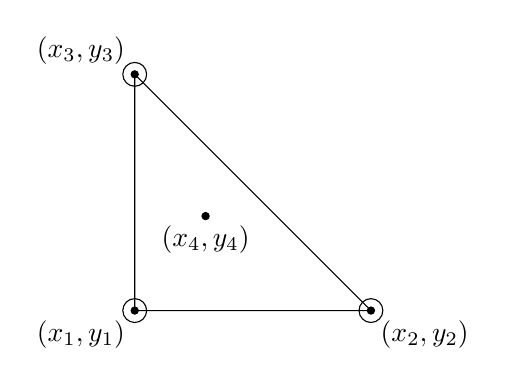
\begin{tikzpicture}
		\draw node[anchor=north east]{$(x_1,y_1)$} (0,0) --  (3,0) node[anchor=north west]{$(x_2,y_2)$} -- (0,3) node[anchor=south east]{$(x_3,y_3)$} -- (0,0);
		\draw[black,fill=black] (0,0) circle (.3ex);
		\draw[black] (0,0) circle (1ex);
		\draw[black,fill=black] (3,0) circle (.3ex);
		\draw[black] (3,0) circle (1ex);
		\draw[black,fill=black] (0,3) circle (.3ex);
		\draw[black] (0,3) circle (1ex);
		\draw[black,fill=black] (.9,1.2) circle (.3ex) node[anchor=north]{$(x_4,y_4)$};
	\end{tikzpicture}
	
	Let $\{N_1,N_2,...,N_{10}\}$ be a subset of the dual of $P$ defined as follows.
	
	$N_1(f)=f(x_1,y_1); \;\;\; N_2(f)=f(x_2,y_2); \;\;\; N_3(f)=f(x_3,y_3); \;\;\; N_4(f)=f(x_4,y_4); $
	
	$N_5(f)=\frac{\partial f}{\partial x}(x_1,y_1); \;\;\; N_6(f)=\frac{\partial f}{\partial x}(x_2,y_2); \;\;\; N_7(f)=\frac{\partial f}{\partial x}(x_3,y_3);$
	
	$N_8(f)=\frac{\partial f}{\partial y}(x_1,y_1); \;\;\; N_9(f)=\frac{\partial f}{\partial y}(x_2,y_2); \;\;\; N_{10}(f)=\frac{\partial f}{\partial y}(x_3,y_3);$
	
	The nodal basis for $P$ is $\{\phi_1,\phi_2,...,\phi_{10}\}$ such that $N_i(\phi_j)=\delta_{ij} \;\;\; \forall i,j \in \{1,2,...,10\}$.
	
	To find a $\phi_l$ as follows. $$\phi_l(x,y)=a_1 x^3+a_2 x^2 y+a_3 x y^2+a_4 y^3+a_5 x^2+a_6 xy+a_7 y^2+a_8 x+a_9 y+a_{10}$$
	
	We solve the following.
	$$
	\begin{bmatrix}
	x_1^3 & x_1^2 y_1& x_1 y_1^2& y_1^3& x_1^2& x_1y_1& y_1^2& x_1& y_1& 1\\[0.15cm]
	x_2^3 & x_2^2 y_2& x_2 y_2^2& y_2^3& x_2^2& x_2y_2& y_2^2& x_2& y_2& 1\\[0.15cm]
	x_3^3 & x_3^2 y_3& x_3 y_3^2& y_3^3& x_3^2& x_3y_3& y_3^2& x_3& y_3& 1\\[0.15cm]
	x_4^3 & x_4^2 y_4& x_4 y_4^2& y_4^3& x_4^2& x_4y_4& y_4^2& x_4& y_4& 1\\[0.15cm]
	
	3x_1^2 & 2x_1y_1 & y_1^2& 0& 2x_1& y_1& 0& 1& 0& 0\\[0.15cm]
	3x_2^2 & 2x_2y_2 & y_2^2& 0& 2x_2& y_2& 0& 1& 0& 0\\[0.15cm]
	3x_3^2 & 2x_3y_3 & y_3^2& 0& 2x_3& y_3& 0& 1& 0& 0\\[0.15cm]
	
	0 & x_1^2 & 2x_1 y_1& 3y_1^2& 0& x_1& 2y_1& 0& 1& 0\\[0.15cm]
	0 & x_2^2 & 2x_2 y_2& 3y_2^2& 0& x_2& 2y_2& 0& 1& 0\\[0.15cm]
	0 & x_3^2 & 2x_3 y_3& 3y_3^2& 0& x_3& 2y_3& 0& 1& 0\\[0.15cm]
	\end{bmatrix}
	\begin{bmatrix} a_1\\[0.15cm]a_2\\[0.15cm]a_3\\[0.15cm]a_4\\[0.15cm]a_5\\[0.15cm]a_6\\[0.15cm]a_7\\[0.15cm]a_8\\[0.15cm]a_9\\[0.15cm]a_{10} \end{bmatrix}
	=\begin{bmatrix} 0 \\[.15cm]0\\[.15cm]0\\[.15cm]1 \\[.15cm]0\\[.15cm]0\\[.15cm]0\\[.15cm]0\\[.15cm]0\\[.15cm]0 \end{bmatrix}
	$$
	The square matrix $M$ is same for all $\phi_l$.
	So we need to calculate the inverse of $M$ only once. After that, we can get the coefficients of the polynomial $\phi_l$ by taking the $l^{th}$ column of the inverse matrix.
	$$
	[a_i]_{10\times 1}=M^{-1} [\delta_{il}]_{10\times 1}=\mbox{ the }l^{th}\mbox{ column of }M^{-1}
	$$
	Program for finding $M$:
	\begin{lstlisting}
		for i in {1,...,10}
		.	(x,y) = location(N_i)
		.	j = 0
		.	for d in {0,...,3}:
		.	.	for px in {0,...,d}:
		.	.	.	if i <= 4
		.	.	.	.	M(i,10-j) = x^(px) * y^(d-px)
		.	.	.	else if i <= 7
		.	.	.	.	if px == 0
		.	.	.	.	.	M(i,10-j) = 0
		.	.	.	.	else
		.	.	.	.	.	M(i,10-j) = px * x^(px-1) * y^(d-px)
		.	.	.	else
		.	.	.	.	if d-px == 0
		.	.	.	.	.	M(i,10-j) = 0
		.	.	.	.	else
		.	.	.	.	.	M(i,10-j) = (d-px) * x^(px) * y^(d-px-1)
		.	.	.	j = j+1
	\end{lstlisting}
	
	For an illustration, if $(x_1,y_1)=(0,0)$, $(x_2,y_2)=(1,0)$, $(x_3,y_3)=(0,1)$, $(x_4,y_4)=(0.3,0.4)$ we get the following matrix $M$.
	$$
	\begin{bmatrix}
	0 & 0 & 0 & 0 & 0 & 0 & 0 & 0 & 0 & 1 \\
	1 & 0 & 0 & 0 & 1 & 0 & 0 & 1 & 0 & 1 \\
	0 & 0 & 0 & 1 & 0 & 0 & 1 & 0 & 1 & 1 \\
	0.027 & 0.036 & 0.048 & 0.064 & 0.09 & 0.12 & 0.16 & 0.3 & 0.4 & 1.0 \\
	0 & 0 & 0 & 0 & 0 & 0 & 0 & 0 & 0 & 1 \\
	3 & 0 & 0 & 0 & 2 & 0 & 0 & 1 & 0 & 0  \\
	0 & 0 & 1 & 0 & 0 & 1 & 0 & 1 & 0 & 0  \\
	0 & 0 & 0 & 0 & 0 & 0 & 0 & 1 & 0 & 0  \\
	0 & 1 & 0 & 0 & 0 & 1 & 0 & 0 & 1 & 0  \\
	0 & 0 & 0 & 3 & 0 & 0 & 2 & 0 & 1 & 0  \\
	\end{bmatrix}
	$$
	
	
	For the $N_5,...,N_{10}$, instead of taking derivatives along the $x$ and $y$ axis, we can take them along other directions. For triangles whose one or more edges lie on $\Gamma \subset \partial \Omega$, we can take the nodes such that for each edge lying on $\Gamma \subset \partial \Omega$, apart from the two nodes that evaluate the function on the end point of the edges, two nodes should evaluate the directional derivate of the function along the edge at different points.
	For example, in the given diagram, if the edge joining $(x_1,y_1)$ and $(x_2,y_2)$ lies in $\Gamma \subset \partial \Omega$ , which is the part on which the Dirichlet condition needs to be satisfied, the following conditions will ensure that a function $f$ is zero on that edge.
	$$N_1(f)=0;\;\;\;N_2(f)=0;\;\;\;N_5(f)=0;\;\;\;N_6(f)=0$$
	
	Thus all, except the following, are free nodes:
	\begin{itemize}
  \item Nodes which evaluate the function on a point in $\Gamma$,
  \item Nodes which evaluate the partial derivative of the function on a point in $\Gamma$, along a direction tangential to $\Gamma$.
	\end{itemize}
  Note that for a given triangulation, nodes which lie on the edges may be shared across multiple triangles. Let $\{N_i\}$ be the set of all the nodes in the triangulation $T_h$ . Then, we define the approximation space. $$V_h=\{v \in C^0(\Omega) \mbox{ such that }\left.v\right|_K \in P\;\;\forall\;K\in T_h\mbox{ and }\left.v\right|_{\Gamma}=0\}$$
  The following set can be proved to be a basis of $V_h$.
  \begin{equation*}
	\begin{split}
  \{ \;\;v\in  C^0(\Omega) \mbox{ such that }\left.v\right|_K \in P\;\;\forall\;K\in T_h\mbox{ and }  \exists\; l  \mbox{ such that }\;\; \\ N_l\mbox{ is a free node and } N_l(v)=1 \mbox{ and }N_i(v)=0 \;\;\forall\;i\neq l \;\;\;\;\;\}
  \end{split}
  \end{equation*}
\end{document}
